\subsection{Deep Neural Network architectures for for Analysis of Sound Scenes and Events}

%\textbf{ndRob} to complete, 3 pages with figures
%\begin{itemize}
%\item formula (notazione matriciale) del calcolo output di ogni rete
%\end{itemize}

A \textit{biological Neural Networks} is a big set of specialized cells (\textit{neurons}) connected among them, which memorize and process information, thus controlling the body activities they belong to.

\begin{figure}[t]
\centering
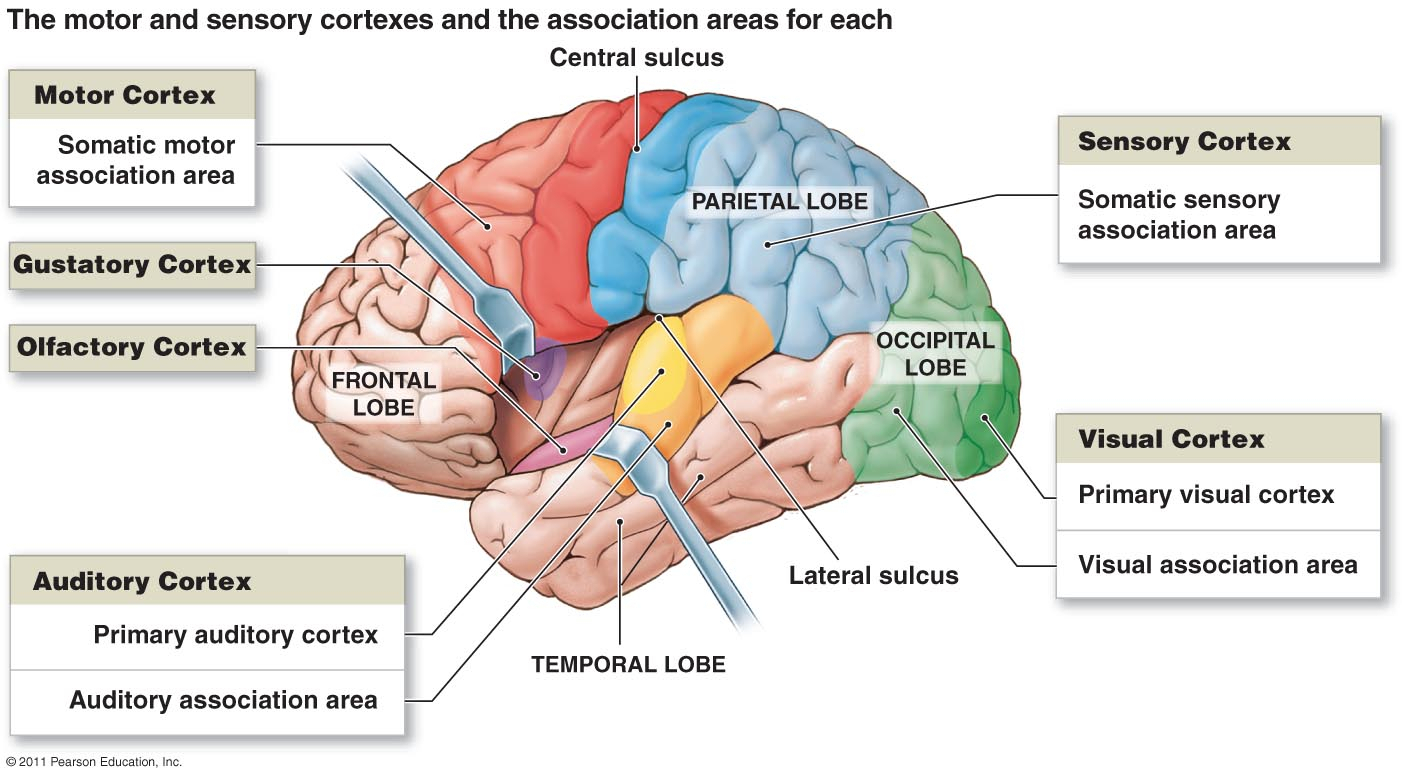
\includegraphics[width=0.65\linewidth]{img/Brain}
\caption{The human brain.}
%\label{vv}
\end{figure}

The \textit{neuron} model is composed of:
\begin{itemize}
\item DENDRITE: input terminal
\item CELL BODY (Nucleus): processing core
\item AXON: output way-out
\item SYNAPSES: output terminal (with weight)
\end{itemize}

%The Biological neurons are electro-chemical devices, operating at low rates ($\approx mses$).
%Digital circuits operate at very high rates ($\approx nsec$).

\begin{figure}[t]
\centering
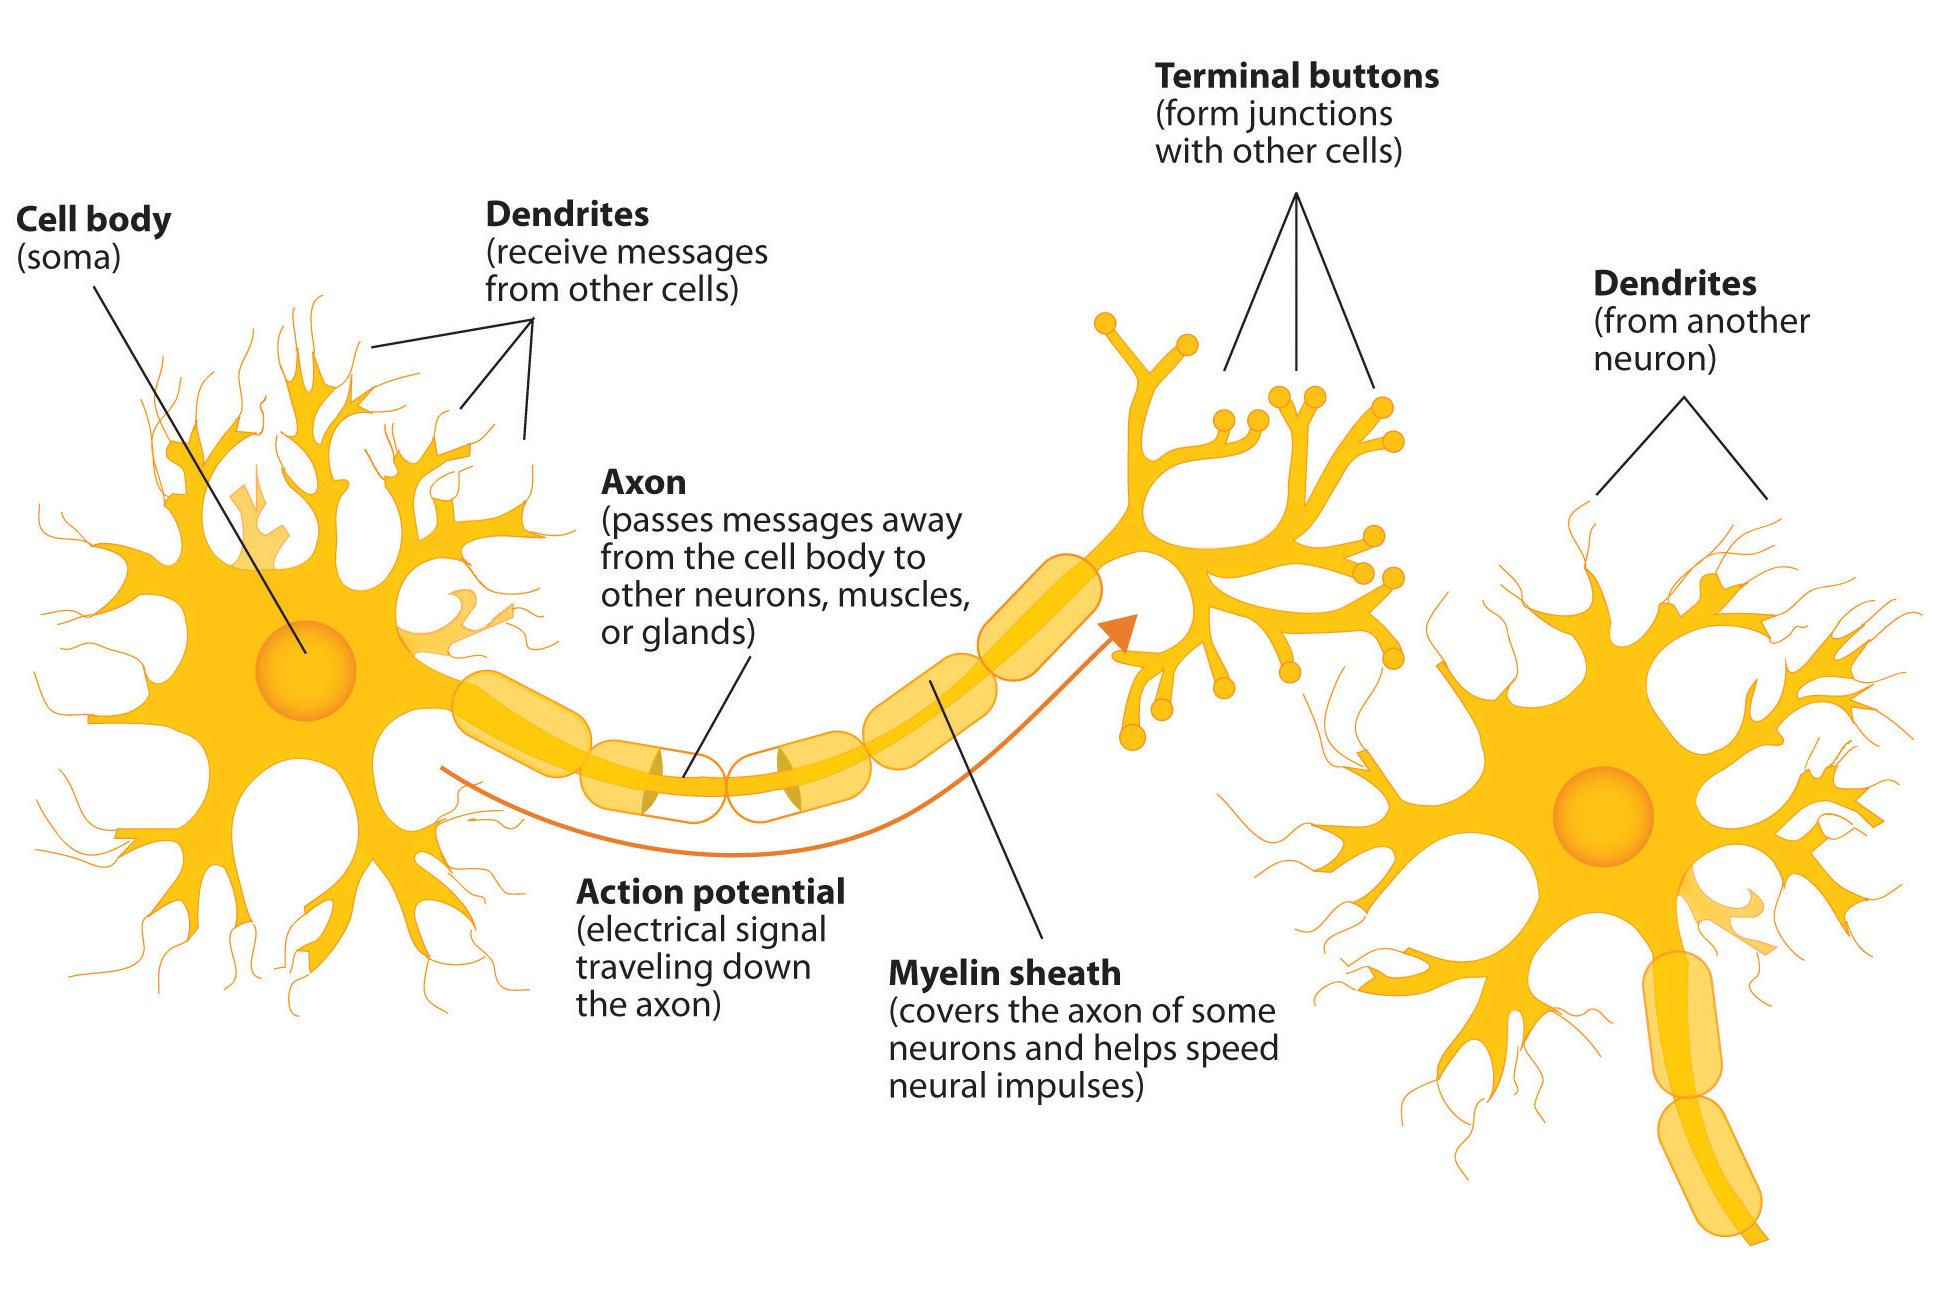
\includegraphics[width=0.4\linewidth]{img/neuron_model}
\caption{The neuron model.}
%\label{aa}
\end{figure}

The \textit{neuron} properties can be described in:
\begin{itemize}
\item LOCAL SIMPLICITY: the neuron receives stimuli (excitation or inhibition) from dendrites and produces an impulse to the axon which is proportional to the weighted sum of the inputs;
\item GLOBAL COMPLEXITY: the human brain possess 
$\mathcal{O}(10^{10})$ 
neurons, with more than 10K connections each;
\item LEARNING: even though the network topology is relatively fixed, the strength of connections (synaptic weights) can change when the network is exposed to external stimuli;
\item DISTRIBUTED CONTROL: no centralized control, each neuron reacts only to its own stimuli;
\item TOLERANCE TO FAILURES: performance slowly decrease with the increase of failures.
\end{itemize}

The biological Neural Networks are able to solve very complex tasks in few time instants (like memorization, recognition, association, and so on.)

\begin{figure}[t]
\centering
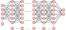
\includegraphics[width=0.4\textwidth]{img/ANN}
\caption{The Artificial Neural Network.}
%\label{aa}
\end{figure}

The \textit{Artificial Neural Networks} (ANNs) are defined as \textit{Massively parallel distributed processors made up of simple processing units having a natural propensity for storing experiential knowledge and making it available for use} (Haykin, 2008).

An ANN resembles the brain in two aspects:
\begin{enumerate}
\item Knowledge is acquired by the network from its environment through a learning process;
\item Synaptic weights are used to store the acquired knowledge.
\end{enumerate}

A \textit{neuron} is an information-processing unit that is fundamental to the operation of a neural network.
The model of a neuron is composed of three basic elements of the neural model:
\begin{itemize}
\item a \textit{set of synapses}, or connecting links, each of which is characterized by a weight or strength of its own, $w_{kj}$;
\item an \textit{adder} for summing the input signals, weighted by the respective synaptic strengths of the neuron; the operations described here constitute a linear combiner;
\item an \textit{activation function} for limiting the amplitude of the output of a neuron. Typically, the normalized amplitude range of the output of a neuron is written as the closed unit interval [0,1], or, alternatively, [-1,1].
\end{itemize}
The neural model also includes an externally applied \textit{bias}, denoted by $b_k$.

\begin{figure}[t]
\centering
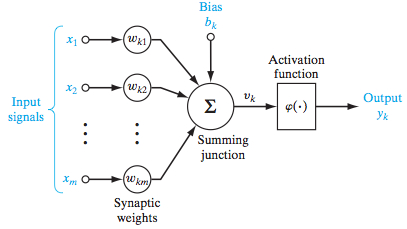
\includegraphics[width=0.8\linewidth]{img/NeuronModel.jpg}
%\label{aa}
\caption{The artificial neuron model.}
\end{figure}

Therefore, the mathematical description of neuron activity can be defined as:
\begin{eqnarray}
{ u }_{ k }=\sum _{ j=1 }^{ m }{ { w }_{ kj } } { x }_{ j }\\ 
{ y }_{ k }=\varphi \left( { u }_{ k }+b_{ k } \right)
\end{eqnarray}
where:
\begin{itemize}
\item ${ x }_{ 1 },{ x }_{ 2 },\cdots ,{ x }_{ m }$ are the input signals;
\item ${ w }_{ k1 },{ w }_{ k2 },\cdots ,{ w }_{ km }$ are the respective synaptic weights of neuron $k$;
\item $u_k$ is the linear combiner output due to the input signals;
\item $b_k$ is the bias;
\item $\varphi(\cdot)$ is the activation function;
\item $y_k$ is the output signal of the neuron.
\end{itemize}

The types of \textit{activation non-linear functions} $\varphi(x)$ are:
\begin{itemize}

\item the \textit{threshold function}: in engineering, this form of a threshold function is commonly referred to as a Heaviside function;
\begin{eqnarray}
\varphi \left( v \right) =1\quad if\quad v\ge 0 \\ 
\varphi \left( v \right) =0\quad if\quad v<0
\end{eqnarray}
\begin{figure}
\centering
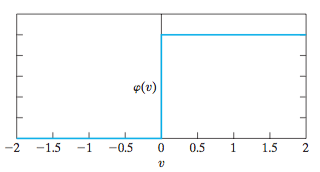
\includegraphics[width=0.4\textwidth]{img/Heaviside}
\caption{The threshold non-linear function.}
%\label{aa}
\end{figure}

\item the \textit{sigmoid function}: it is defined as a strictly increasing function that exhibits a graceful balance between linear and nonlinear behavior; an example of the sigmoid function is the \textit{logistic function} defined by:
\begin{equation}
\varphi \left( v \right) =\frac { 1 }{ 1+exp\left( -av \right)  } 
\end{equation}
\begin{figure}
\centering
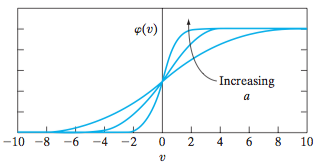
\includegraphics[width=0.4\textwidth]{img/sigmoid}
\caption{The sigmoid non-linear function.}
%\label{aa}
\end{figure}

\item the \textit{ hyperbolic tangent } ($tanh$): it is simply a scaled and shifted version of the sigmoid function:
\begin{equation}
\varphi(x) = \frac{1-e^{-2x}}{1+e^{-2x}}
\end{equation}
\begin{figure}[t]
\centering
	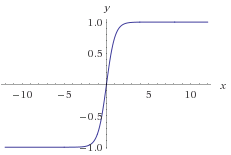
\includegraphics[width=0.4\textwidth]{img/tanh}
	\caption{The $tanh$ non-linear function.}
%				\label{aa}
\end{figure}

\item the \textit{ Rectifier Linear Unit} ($ReLU$):
\begin{equation}
\varphi(x) = \text{max}(0,x)
\end{equation}
\begin{figure}[t]
\centering
	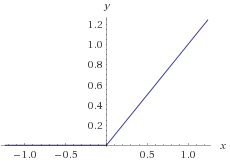
\includegraphics[width=0.4\textwidth]{img/relu}
	\caption{The $ReLU$ non-linear function.}
%				\label{ee}
\end{figure}

\item the $softmax$: it is used on the last layer of a classifier setup: the outputs of the softmax layer represent the probabilities that a sample belongs to the different classes. Indeed, the sum of all the output is equal to $1$.
			%In this case the targets are \textit{one-hot} vectors and the cost-function is the \textit{categorical cross-entropy}.
\begin{equation}
\varphi(x_k) = \frac{e^{x_k}}{\sum_{j=1}^{N}e^{x_j}} \text{ for }  k=1,\dots,K
\end{equation}
\begin{figure}[t]
\centering
	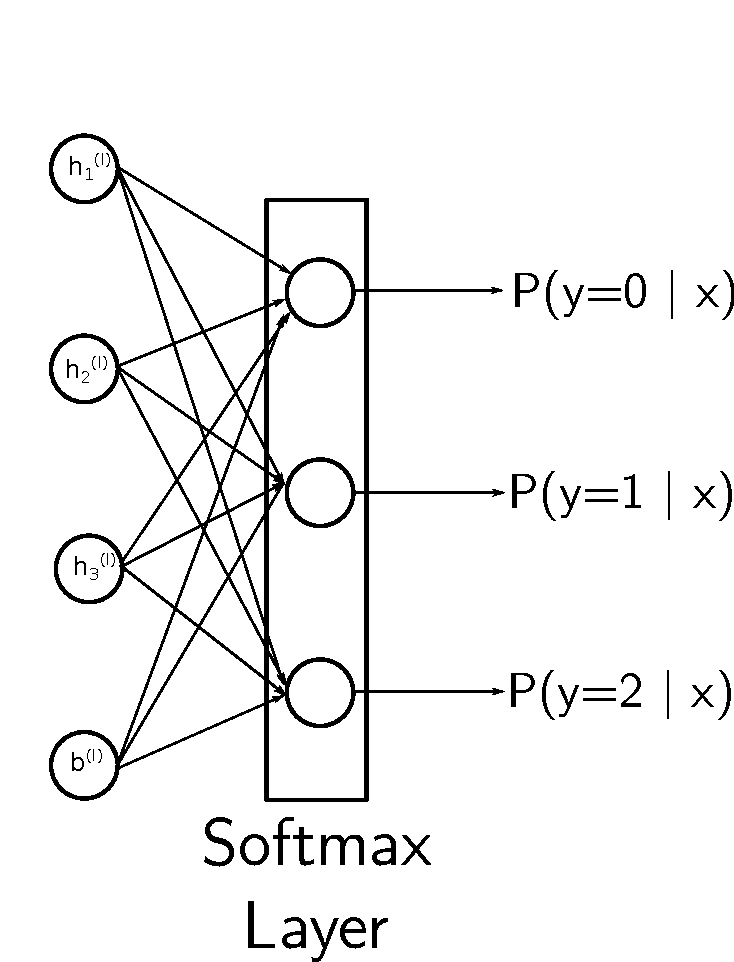
\includegraphics[width=0.4\textwidth]{img/softmax}
	\caption{The $\textit{softmax}$ layer in a neural network classifier.}
%					\label{aa}
\end{figure}	
			
%			\item $\mathbf{maxout}$ - the output is the maximum value among $K$ linear models applied to a given input (or an hidden activation): $\varphi(x_k) = \max(x_k)$ with $k=1,\dots,K$.\\
%			It is supposed to be combined with dropout.
			
	%		It is an approximate model averaging technique. A single maxout unit performs a piecewise linear approximation to an arbitrary convex function. Maxout networks learn not just the relationship between hidden units, but also the activation function of each hidden unit.	
		
				
		
%				\begin{figure}
%				\centering
%					\includegraphics[width=0.75\textwidth]{img/maxout}
%					\caption{Example of an MLP with $\mathbf{maxout}$ units. Picture courtesy of GoodFellow et al. 2013}
%%					\label{rr}
%				\end{figure}

\end{itemize}

% ****************************************************+
%NEURAL NETWORKS VIEWED AS DIRECTED GRAPHS
%
%A neural network is a \textbf{directed graph} consisting of nodes with interconnecting synaptic and activation links and is characterized by four properties:
%
%\begin{enumerate}
%\item Each neuron is represented by a set of linear synaptic links, an externally applied bias, and a possibly nonlinear activation link. The bias is represented by a synaptic link connected to an input fixed at $+1$.
%\item The synaptic links of a neuron weight their respective input signals.
%\item The weighted sum of the input signals defines the induced local field of the neuron in question
%\item The activation link squashes the induced local field of the neuron to produce an output
%\end{enumerate}
%
%\begin{figure}
%\centering
%\includegraphics[width=0.55\textwidth]{img/NeuronGraph.jpg}
%\caption{The Neuron graph model.}
%%\label{key}
%\end{figure}
%
%When the focus of attention is restricted to signal flow from neuron to neuron, we may use a reduced form of this graph by omitting the details of signal flow inside the individual neurons. Such a directed graph is said to be \textit{partially complete}. It is characterized as follows:
%
%\begin{enumerate}
%\item Source nodes supply input signals to the graph.
%\item Each neuron is represented by a single node called a computation node.
%\item The communication links interconnecting the source and computation nodes of the graph carry no weight; they merely provide directions of signal flow in the graph.
%\end{enumerate}
%
%%\begin{figure}
%%\centering
%%\includegraphics[width=0.55\textwidth]{img/NeuronPGraph.jpg}
%%%\label{aa}
%%\caption{ee}
%%\end{figure}
%
%
%Graphical representations of a neural network
%
%\begin{itemize}
%\item \textbf{Block Diagram} $\rightarrow$ functional description of the network
%\item \textbf{Architectural Graph} $\rightarrow$ description of the network layout
%\item \textbf{Signal-Flow Graph} $\rightarrow$ complete description of the signal flow in the network
%\end{itemize}

% *********************************************************+

The manner in which the neurons of a neural network are structured is intimately linked with the learning algorithm used to train the network. % Therefore, the learning algorithms (rules) used in the design of neural networks as being structured.
There, the \textit{network architectures} (structures) is defined.
In general, two different classes of network architectures are identified:
\begin{enumerate}

%\item \textit{Single-Layer Feedforward Networks} (SLFN):
%
%\begin{itemize}
%\item We have an input layer of source nodes that projects directly onto an output layer of neurons (computation nodes), but not vice-versa 
%\item Such a network is called a single-layer network, with the designation \emph{single-layer} referring to the output layer of computation nodes (neurons). 
%\item We do not count the input layer of source nodes because no computation is performed there.
%\end{itemize}
%
%\begin{figure}
%\centering
%\includegraphics[width=0.35\textwidth]{img/SLFN}
%%\label{aa}
%\caption{The Single-Layer Feedforward Network.}
%\end{figure}


\item \textit{Multilayer Feedforward Networks} - (FFNN):

it is characterized by the presence of one or more hidden layers, whose computation nodes are correspondingly called \textit{hidden neurons} (or hidden units);
the term \textit{hidden} refers to the fact that this part of the neural network is not seen directly from either the input or output of the network. 
The function of hidden neurons is to intervene between the external input and the network output in some useful manner. By adding one or more hidden layers, the network is enabled to extract higher-order statistics from its input. 
%\item Example: \textbf{10-4-2 network} $->$ it has 10 source nodes, 4 hidden neurons, and 2 output neurons.


\begin{figure}
\centering
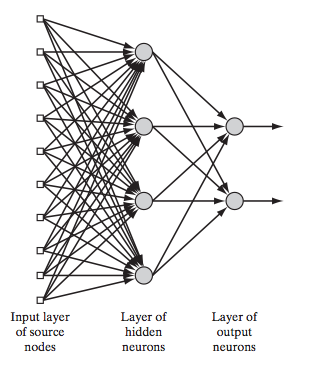
\includegraphics[width=0.4\textwidth]{img/MLP}
%\label{aa}
\caption{The Multilayer Feedforward Network.}
\end{figure}


%\textbf{ndRob} to complete, 1 pages with figure
%\begin{itemize}
%\item struttura a layer
%\item notazione matriciale con indici layer
%\end{itemize}

The MLP is a well known kind of artificial neural network introduced in 1986 \cite{Rumelhart86-LRB}. 
Each node applies an activation function over the weighted sum of its inputs. 
The units are arranged in layers, with feed forward connections from one layer to the next. 
The stochastic gradient descent with error back-propagation algorithm is used for the supervised learning of the network. 
In the forward pass, input examples are fed to the input layer, and the resulting output is propagated via the hidden layers towards the output layer. At the backward pass, the error signal originating at the output neurons is sent back through the layers and the network parameters (i.e., weights and biases) are tuned.

A single neuron can be formally described as:
\begin{equation}
%g(\mathbf{u}[n])=\varphi \left(\left(\begin{matrix} \sum _{ j=1 }^{ D }{w_j u_j[n] }  \end{matrix} \right) + b\right),
g(\mathbf{u}[n])=\varphi \left(\sum _{ j=1 }^{ D }{w_j u_j[n] } + b\right),
\end{equation}
where $\mathbf{u}[n] \in \mathbb{R}^{D\times 1}$, the bias $b$ is an externally applied term and $\varphi(\cdot)$ is the non-linear activation function.
Thus, the mathematical description of a one-hidden-layer MLP is a function $\mathbf{f}:\mathbb{R}^D \rightarrow \mathbb{R}^{D'}$, where $D'$ is the size of the output vector, so:
\begin{equation}
\mathbf{f}(\mathbf{u}[n]) = 	\varphi \left( \mathbf{b}_2 + \mathbf{W}_2 \left( \varphi \left( \mathbf{b}_1 + \mathbf{W}_2 \cdot \mathbf{u}[n]\right) \right) \right),
\end{equation}
where $\mathbf{W}_i$ and $\mathbf{b}_{i}$ are the respective synaptic weights matrix and the bias vector of the $i$-th layer.
The behaviour of this architecture  is  parametrized  by  the connection weights, which are adapted during the supervised network training.



\item \textit{Convolutional Neural Networks}(CNN)

\begin{figure}
	 \centering
	 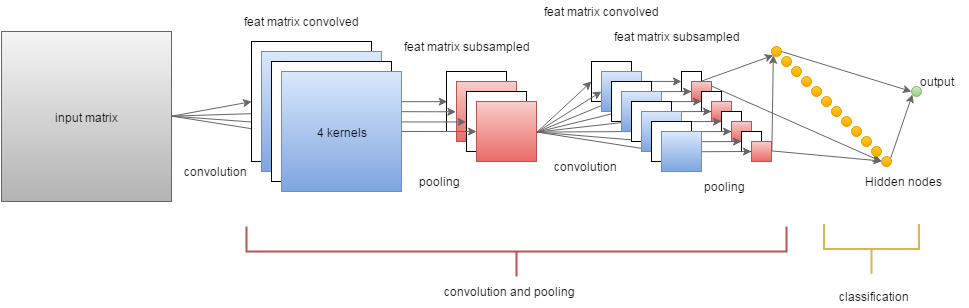
\includegraphics[width=0.9\columnwidth]{img/CNN}
%	 \label{ee}
	 \caption{The Convolutional Neural Network.}
	\end{figure}

%\textbf{ndRob} to complete,  1 pages with figure

Convolutional neural networks are feedforward neural networks similar to multilayer perceptron, with some special layers.

%Matrix convolution: it is performed between a bigger matrix, which is the input, and a smaller matrix, the convolutional kernel.

\begin{figure}[t]
		\centering
		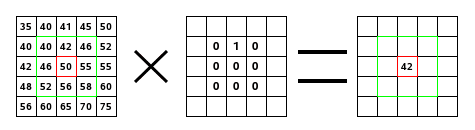
\includegraphics[width=0.7\columnwidth]{img/convolution-calculate}
%		\label{ee}
		\caption{The convolution operation.}
	\end{figure}
	


%	\item Convolution kernels, by training, adapt on recurrent input patterns, becoming themselves similar to those patterns. As a result an activation of the kernel is given when a specific pattern occurs. 
Convolution kernels process the input data matrix by dividing it in \textit{local receptive fields}, a region of the same size of the kernel, and sliding the local receptive field across the entire input.
Each hidden neuron is thus connected to a local receptive field, and all the neurons form a matrix called \textit{feature map}.
%We can have multiple feature maps.
The weights in each \textit{feature map} are \textit{shared}: all hidden neurons are aimed to detect exactly the same pattern just at different locations in the input image. 

The main advantages of this network is the robust pattern recognition system characterized by a strong immunity to pattern shifts.

Pooling layer just reduces the dimension of the matrix by a rule: a submatrix of the input is selected, and the output is the maximum value of this submatrix.
	
	\begin{figure}
		\centering
		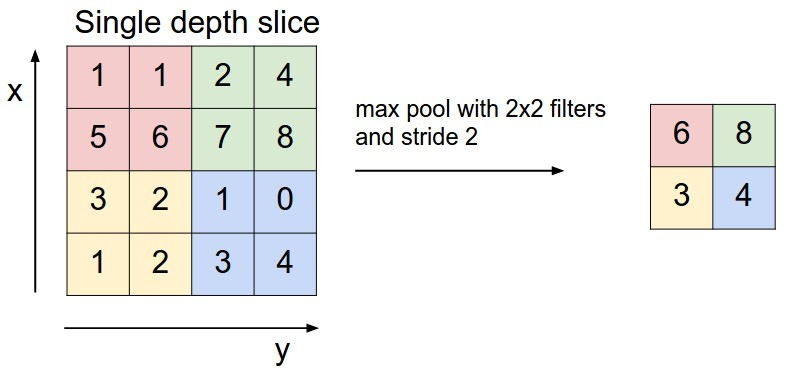
\includegraphics[width=0.6\columnwidth]{img/maxpool.jpeg}
%		\label{rr}
		\caption{The max-pooling layer.}
	\end{figure}

The pooling process introduces tolerance against shifts of the input patterns. Together with convolution layer it allows the CNN to detect if a particular event occurs, regardless its deformation or its position.

CNN is a feed-forward neural network \cite{726791} usually composed of three types of layers: convolutional layers, pooling layers and layers of neurons.
The convolutional layer performs the mathematical operation of convolution between a multi-dimensional input and a fixed-size kernel. Successively, a non-linearity is applied element-wise. 
%In the convolution process the kernel moves all along the input matrix and, for each position, every element of the kernel is multiplied with the corresponding one on the input matrix. All the values are finally summed.
The kernels are generally small compared to the input, allowing CNNs to process large inputs with few trainable parameters.
%From the input matrix, for each convolutional kernel, a new matrix is obtained, also called \textit{feature map}.
Successively, a pooling layer is usually applied, in order to reduce the feature map dimensions. One of the most used is the \textit{max-pooling} whose aim is to introduce robustness against translations of the input patterns.
%Different strategies are available for pooling, but we only consider max-pooling, which selects the maximum value in a sub-matrix of the input and discards the other values. Pooling introduces toughness against shifts of the input patterns. 
Finally, at the top of the network, a layer of neurons is applied. This layer does not differ from MLP, being composed by a set of activation and being fully connected with the previous layer. For clarity, the units contained in this layer will be referred as \textit{Hidden Nodes} (HN).

Denoting with $\mathbf{W}_{m} \in \mathbb{R}^{K_{1m}\times K_{2m}}$ the $m$-th kernel and with $\mathbf{b}_{m}  \in \mathbb{R}^{D_1\times D_2}$ the bias vector of a generic convolutional layer, the $m$-th feature map  $\mathbf{h}_{m} \in \mathbb{R}^{D_1\times D_2}$ is given by:
\begin{equation}\label{eq:backg:dnn:conv_op}
%h_{m,i}=\varphi	\left(W_{m,i} \ast \mathbf{u}_j[n] + b_{m,i} \right),
\mathbf{h}_{m}=\varphi	\left(\sum_{d=1}^{D_3} \mathbf{W}_{m} \ast \mathbf{u}_d + \mathbf{b}_{m} \right),
\end{equation}
where $\ast$ represent the convolution operation, and $\mathbf{u}_{d} \in \mathbb{R}^{D_1\times D_2} $ is a matrix of the three-dimensional input tensor $\mathbf{u} \in \mathbb{R}^{D_1\times D_2 \times D_3}$. The dimension of the $m$-th feature map $\mathbf{h}_{m}$ depends on the zero padding of the input tensor: here, padding is performed in order to preserve the dimension of the input, i.e., $\mathbf{h}_{m} \in \mathbb{R}^{D_1\times D_2}$. Please note that for the sake of simplicity, the time frame index $n$ has been omitted.  %The different feature maps obtained from each kernel of a convolutional layer are then summed to compose the input data for the following layer.
Commonly, \eqref{eq:backg:dnn:conv_op} is followed by a pooling layer in order to be more robust against patterns shifts in the processed data, e.g. a max-pooling operator that calculates the maximum over a $P_1 \times P_2 $ matrix is employed.

\end{enumerate}


A \textit{Deep Learning} definition: \textit{A  class  of  machine learning  techniques  that
exploit  many  layers  of  non-linear  information  processing  for supervised  or  unsupervised  feature  extraction  and  transformation, and for pattern analysis and classification.}
%...we need complex networks to deal with the \textit{feature representation learning} paradigm.
Artificial Neural Networks are often referred as deep when they have more than 1 or 2 hidden layers.
%		\item Important Issues
%		\begin{itemize}
%			\item Rule of Thumb: \textit{for a given performance rate on the testing data, the amount of training data and the number of free parameters are directly proportional}.
%			\item Do we have enough data for training and to achieve a satisfying generalization performance?
%			\item How to select the ``right'' model? 
%		\end{itemize}


\subsection{Stochastic gradient descent (SGD)}

Most deep learning training algorithms involve optimization of some sort.
The most widely used is the gradient based optimization, which belongs to the first order type.

\textit{Optimization} is the task of either minimizing some function $f(x)$ by altering $x$:
$f(x)$ is called \textit{objective function}, but in the case when it has to be minimized, it is also call the \textit{cost function}, \textit{loss function}, or \textit{error function}.
The aim of the optimization is reached doing small change $\epsilon$ in the input $x$, to obtain the corresponding change in the output $f(x)$:
\begin{equation}
f(x+\epsilon) \approx f(x)+\epsilon\,f'(x).
\end{equation}
This formulation is based on the calculation of the derivative $f'(x)$.
The \textit{gradient descent} is the technique based on the reduction of $f(x)$ by moving $x$ in small steps with the opposite sign of the derivative.
The aim is to find the minimum of the cost function: when $f'(x)=0$, the derivative provides no information about which direction to move, therefore this point is defined as stationary points.
A local minimum is a point where $f(x)$ is lower than at all neighbouring and it is no longer possible to decrease $f(x)$ by making infinitesimal steps.
The absolute lowest value of $f(x)$ is a \textit{global minimum}.

For the concept of minimization to make sense, there must still be only one (scalar) output.
For functions that have multiple inputs $f: \R^n \rightarrow \R$, the concept of \textit{partial derivatives} is introduced.
The gradient $\nabla_{\mathbf{x}}f(\mathbf{x})$ is the vector containing all the partial derivatives.

The method of \textit{steepest descent} or \textit{gradient descent} states that decrease $f$ by moving in the direction of the negative gradient.
\begin{equation}
\textbf{x'} = \textbf{x} - \epsilon\,\nabla_{\mathbf{x}}f(\mathbf{x}),
\end{equation}
where $\epsilon$ is the \textit{learning rate}, a positive scalar determining the size of the step.

Large training sets are necessary for good generalization, but large training sets are also more computationally expensive.
The cost function decomposes as a sum over training example of per-example loss function:
i.e., the negative conditional log-likelihood of the training data is defined as:
\begin{equation}
J(\mathbf{\theta}) = \mathbb{E}(L(\textbf{x}, y, \mathbf{\theta})) = \frac{1}{m} \sum\limits_{i=1}^{m} L(\textbf{x}^{(i)}, y^{(i)}, \mathbf{\theta}),
\end{equation}
where $L$ is the per-example loss $L(\textbf{x}, y, \mathbf{\theta}) = - \log p(y|\textbf{x};\mathbf{\theta})$.
The gradient descent requires computing:
\begin{equation}
\nabla_{\theta} J(\mathbf{\theta}) = \frac{1}{m} \sum\limits_{i=1}^{m} \nabla_{\theta} L(\textbf{x}^{(i)}, y^{(i)}, \mathbf{\theta}).
\end{equation}
The computational cost of this operation is proportional to the number of example $m$, therefore as the training set size grows the time to take a single gradient step becomes prohibitively long.

\textit{Stochastic gradient descent} (SGD) is an extension of the gradient descent algorithm: the insight is that the gradient is an expectation estimated using a small set of samples.
On each step of the algorithm, a sample of example $\mathbb{B} = \{ \textbf{x}^{(1)}, \ldots, \textbf{x}^{(m')}\}$, called \textit{minibatch}, is drawn uniformly from the training set.
The minibatch size $m'$ is typically chosen to be a relatively small number of examples.
The estimate of the gradient is:
$\textbf{g} = \frac{1}{m'} \nabla_{\theta} \sum\limits_{i=1}^{m'} L(\textbf{x}^{(i)}, y^{(i)}, \mathbf{\theta})$
using examples from the minibatch $\mathbb{B}$.
The SGD algorithm then follows the estimated gradient downhill:
\begin{equation}
\theta \leftarrow \theta - \epsilon\,\textbf{g}
\end{equation}
where $\epsilon$ is the learning rate.

%\textbf{ndRob} to be inserted: tipo di loss function MSE, come si calcola su uscita 

%\textbf{ndRob} to complete, learning for FF e CNN (in slides)




\subsection{Autoencoder}

%\textbf{ndRob} to complete, 1-2 pages with figures
%
%\begin{itemize}
%\item definition
%\item notazione matriciale
%\item denoising Auto Encoder (dAE)
%\end{itemize}



An Autoencoder is a kind of neural network typically consisting of only one hidden layer, trained to set the target values to be equal to the inputs.
\begin{equation} %\label{eq:layer2}
  \tilde{x} = f(W_{2}h(x) +b_{2})
\end{equation}
 
%\begin{figure}
%\centering
%\includegraphics[width=0.65\textwidth]{img/basic_AE}
%%\label{ee}
%\caption{rr}
%\end{figure}


Given an input set of examples $\mathcal{X}$, autoencoder training consists
in finding parameters $\theta=\{W_{1},W_{2},b_{1},b_{2}\}$ that
minimize the Reconstruction Error:
\begin{equation}\label{eq:obAE}
  \mathcal{J}(\theta)=\sum_{x\in{\mathcal{X}}}\left\| x - \tilde{x}\right\|^{2}
\end{equation}

Defining $M$ the number of hidden units, and $N$ the number of input units, output units, features size:

\begin{figure}
\centering
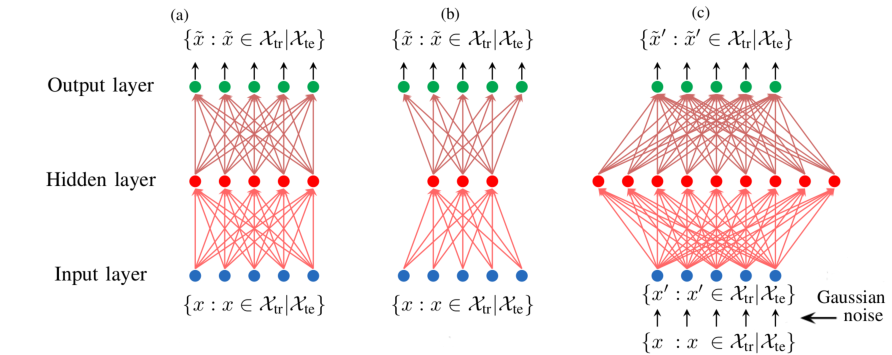
\includegraphics[width=\columnwidth]{img/autoencoders}
\caption{The different types of Autoencoders.}
\label{fig:backg:dnn:AE}
\end{figure}

\begin{itemize}
\item (a):  $M=N \rightarrow$ Basic Autoencoder (AE);
\item (b):  $M<N \rightarrow$ Compression Autoencoder (CAE);
\item (c):  $M>N$ and Gaussian Noise $\rightarrow$ Denoising Autoencoder (DAE);
\end{itemize}


%This section introduces the concepts of autoencoders and describes the basic autoencoder, compression autoencoder, de-noising autoencoder, and non-linear predictive autoencoder.


\subsubsection{Basic Autoencoder}
A basic AE -- a kind of neural network typically consisting of only one hidden layer --, sets the target values to be equal to the input. It is used to find common data representation from the input \cite{Goodfellow2009-MII,Bengio2007-GLT}. Formally, in response to an input example $x\in \mathbf{R}^{n}$, the hidden representation
$h(x) \in \mathbf{R}^{m}$ is 
\begin{equation} %\label{eq:layer1}
  h(x) = f(W_{1}x +b_{1}), 
\end{equation}
where $f(z)$ is a non-linear activation function, typically a logistic
sigmoid function $f(z) = 1/(1+\exp(-z)) $ applied component-wisely,
$W_{1} \in \mathbf{R}^{m \times n}$ is a weight matrix, and $b_{1} \in
\mathbf{R}^{m}$ is a bias vector.

The network output maps the hidden representation $h$ back to a
reconstruction $\tilde{x} \in \mathbf{R}^{n}$:
\begin{equation} %\label{eq:layer2}
  \tilde{x} = f(W_{2}h(x) +b_{2}), 
\end{equation}
where $W_{2} \in \mathbf{R}^{n \times m}$ is a weight matrix, and $b_{2} \in
\mathbf{R}^{n}$ is a bias vector.

Given an input set of examples $\mathcal{X}$, AE training consists
in finding parameters $\theta=\{W_{1},W_{2},b_{1},b_{2}\}$ that
minimise the reconstruction error, which corresponds to minimising
the following objective function:
\begin{equation} %\label{eq:obAE}
  \mathcal{J}(\theta)=\sum_{x\in{\mathcal{X}}}\left\| x -
    \tilde{x}\right\|^{2}.
\end{equation}
The minimisation is usually realised by stochastic gradient descent as
in the training of neural networks. The structure of the AE is given in \figref{fig:backg:dnn:AE}a.   

\subsubsection{Compression Autoencoder}
In the case of having the number of hidden units $m$ smaller than the number of input units $n$, the network is forced to
learn a compressed representation of the input. For example, if some of the input features are correlated, then this compression autoencoder (CAE) is able to learn those correlations and reconstruct the input data from a compressed representation. The structure of the CAE is given in \figref{fig:backg:dnn:AE}b.

\subsubsection{De-noising Autoencoder}\label{sssec:backg:dnn:dAE}
The de-noising AE (DAE) \cite{Vincent10-SDA} forces the hidden layer to retrieve more robust features and prevent it from simply learning the identity. In such a configuration the AE is trained to reconstruct the original input from a corrupted version of it. Formally, the initial input $x$ is corrupted by means of additive isotropic Gaussian noise in order to obtain: $x'|x \sim N(x,\sigma^2I)$. The corrupted input $x'$ is then mapped, as with the AE, to a hidden representation
\begin{equation} %\label{eq:layer11}
  h(x') = f(W'_{1}x' +b'_{1}), 
\end{equation}
from which the original signal is reconstructed as follows:
\begin{equation} %\label{eq:layer12}
  \tilde{x}' = f(W'_{2}x +b'_{2}). 
\end{equation}
The parameters $\theta'=\{W'_{1},W'_{2},b'_{1},b'_{2}\}$ are trained to minimise the average reconstruction error over the training set, to have $\tilde{x}'$ reach as close as possible to the uncorrupted input $x$, which corresponds to minimising the objective function in Equation \ref{eq:obAE}.
%%%%%%%%%%%%%%%%%%%%%%%%%
The structure of the de-noising autoencoder is shown in \figref{fig:backg:dnn:AE}c.





%\textbf{ndRob} descrizione teorica dAE 1D, from paper Neural NILM, 




